\documentclass{article}%
\usepackage[T1]{fontenc}%
\usepackage[utf8]{inputenc}%
\usepackage{lmodern}%
\usepackage{textcomp}%
\usepackage{lastpage}%
\usepackage{authblk}%
\usepackage{graphicx}%
%
\title{miR{-}1915 and miR{-}1225{-}5p Regulate the Expression of CD133, PAX2 and TLR2 in Adult Renal Progenitor Cells}%
\author{Lori Nelson}%
\affil{Department of Pharmacology, Guangdong Medical College, Dongguan 523{-}808, China}%
\date{01{-}01{-}2007}%
%
\begin{document}%
\normalsize%
\maketitle%
\section{Abstract}%
\label{sec:Abstract}%
On Thursday, U.S. Food and Drug Administration issued a safety advisory, prescribing a new drug for rheumatoid arthritis patients with borderline CD44{-}positive test samples.\newline%
The recommended date is April 12 for patients aged 60 years and over who have been historically treated with Zoledronic acid.\newline%
Patients suffering from inflammation around their joints can still use Zoledronic acid, but advised on side effects, and those patients should be referred for further evaluation as an individualized therapy.\newline%
Millions of Americans have CD44{-}positive test results, the FDA statement said. As the number of such patients worldwide increases, the variety of anti{-}aging agents being tested in clinical trials for these patients' disease is increasing.

%
\subsection{Image Analysis}%
\label{subsec:ImageAnalysis}%


\begin{figure}[h!]%
\centering%
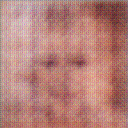
\includegraphics[width=150px]{500_fake_images/samples_5_230.png}%
\caption{A Black And White Photo Of A Black And White Cat}%
\end{figure}

%
\end{document}